%% -*- coding:utf-8 -*-


\chapter{The end of theoretical linguistics? Did I read all this in vain?}
\label{chapter-LLMs}

You read \pageref{last-page-before-LLMs} pages about linguistic theories and may ask yourself:
``Well, we have these great Large Language Models that can do impressive things without making use
of any of the theories laid out in this book, so do we still need linguistic theories? Aren't the
language models better theories of human language? Are all linguistic problems solved? What is the
status of theoretical linguistics, what about its future?'' This issue is also discussed among
theoretical linguists and surprisingly some claim, that Large Language Models (LLMs) are the best
linguistic theory we have or that LLMs are good theories of
acquisition and mental representations \citep{AmbridgeBlything2024a}. The book you just read contains enough information to be
able to enter this discussion. This chapter will explain why LLMs differ fundamentally from the
theories discussed in this book. LLMs are not theories (Section~\ref{sec-Are-LLMs-linghuistic-theories}). Theories about general aspects of the human
brain may have played a role in the development of LLMs, but linguistic theories did not.

Section~\ref{sec-differences-LLMs-humans} shows that LLMs differ in crucial ways from humans when it
comes to structural embedding.

The chapter also discusses \citegen{Piantadosi2024a} claim that LLMs refute Chomskyan approaches to linguistics. I show in
Section~\ref{sec-LLMs-and-language-acquisition} that this is not the case yet, but that Chomskyan
approaches have been refuted earlier as is discussed in many places of this book. The reason why
they could be refuted is that they were linguistic theories, semi-formalized but specific enough to
be falsified.

Section~\ref{sec-linguistic-theories} states what linguistic theories should look like and
%Section~\ref{sec-LLMs-experiments} is a brief comment on using LLMs for linguistic experiments, and
Section~\ref{sec-LLMs-conclusion} concludes the chapter.


\section{Are Large Language Models linguistic theories?}
\label{sec-Are-LLMs-linghuistic-theories}


In a paper in a special issue of Theoretical Linguistics containing ``Reflections on
Theoretical Linguistics'' on the occasion of the 50th anniversary of the journal,
\citet{AmbridgeBlything2024a} claim that ``large language models are better than theoretical
linguists at theoretical linguistics'' (p.\,33). The authors examine the output of an LLM with
regard to the argument structures of verbs, and are impressed that the model predicts the same as
Ambridge found out in experiments with students. The authors claim that LLMs are a theory of
language. The best one we have right now:
\begin{quote}
large language models (LLMs) are already the leading current theories of how speakers learn and
represent these restrictions. Of course, they are not perfect theories [\ldots] but they’re better
theories than any others that have been proposed. \citep[\page 34]{AmbridgeBlything2024a}
\end{quote}
Similarly \citet[360]{Piantadosi2024a} writes:
\begin{quote}
All of this is possible because large language models develop representations
of key structures and dependencies. It's just that these representations are parameterized in a way which is unfamiliar to linguistics. As argued by \citeauthor{Baroni2023a}
(2022), this means that language models should be treated as bona fide linguistic
theories. \citep[360]{Piantadosi2024a}
\end{quote}
% See also Lappin2024a:12
%
LLMs are very interesting and you can do a lot of impressive things with them.\footnote{%
For example, ChatGPT can explain prime factorizations in Trump-style \citep[356--357]{Piantadosi2024a}.
} But are they theories? Do they help in any way to get a better understanding of language?

The authors claim that large language models are theories of language acquisition and representation
and that they are instantiations of Construction Grammar approaches \citep{Goldberg2006a}: 
\begin{quote}
Large language models [...] constitute theories of language acquisition and representation; theories
that instantiate exemplar-, input- and construction-based approaches, though only very
loosely. \citep[\page 33]{AmbridgeBlything2024a}
\end{quote}

\noindent
The authors claim that models are a theory (see also \citealt[360]{Piantadosi2024a}):
\begin{quote}
OK, so the model makes the right predictions but -- we hear you ask -- where is the theory? That's
the point: the model is the theory.
\citep[\page 39]{AmbridgeBlything2024a}
\end{quote}
This shows some confusion in terminology. 
A \emph{theory} contains descriptive and explanatory statements about some part of the reality. It contains
laws about the domain that is described by the theory. A \emph{model} is an abstract representation of the
relevant part of the reality under consideration. A theory can be used to build such models.
A theory should use primitives that are appropriate for a certain domain and it should contain statements about these
primitives.\footnote{
  András Kornai\ia{Kornai, András} (p.c.\,2026) pointed out to me that there are objects for which a theory would have
  to be identical with the modeled object and hence, there would not be any \isi{compression}. \isi{Kolmogorov-random sequence}s are a case at hand. I think it is
  justified to assume that languages are not random sequences.
} Large language models are neuronal nets that have been organized and trained in a
certain way. Nodes of such nets can be examined and we can even find certain information in them
\citep{ManningClarkHewitt2020a,ZhangBowman2018a} but this information is not a theory. The net may
reflect grammatical structures and reject impossible ones, but it does not tell us why this is the case.

Later in the paper and contradicting their earlier claim, the authors argue that the programs that generate the LLMs are a theory:
\begin{quote}
``But'', critics object, ``we have no idea what it's doing'' (e.g., Kodner et al. 2023; Milway
2023). Quite the opposite: Unlike for traditional linguistic theories, every last detail of the
model's assumptions and operation is written out in black and white, in thousands of lines of
computer code. This code is a theory of the acquisition of (among other things) verb argument
structure; it's even -- like traditional linguistic theories -- written in a language, albeit an
artificial programming language, rather than a natural language like English. We know exactly what
the model is doing.  \citep[\page 39--40]{AmbridgeBlything2024a}
\end{quote}
This very quote is an instance of mixing levels. We know what the \emph{code} is doing. We do not
know what the trained net, the model, is doing. This depends on the training data and even if we
knew the training data, we could not predict what specific nodes in the net would do. The issue is
just too complex for us humans and the training data is too vast. This can be compared with Definite
Clause Grammars: this is a notation that can be used to write down phrase structure grammars. Most
Prolog interpreters come with a component that parses such grammars directly (see
\citealt[Chapter~9]{CM2003a} for more information on DCGs and Task~\ref{task-DCG} on
p.\,\pageref{task-DCG} of this book for more information on working with DCGs online). \citet[268--270]{CM2003a}
provide two pages of code for the translation of DCGs into Prolog code. The resulting Prolog program
does Parsing as Deduction. In this case, we know what the code is doing. It reflects our theory
about language. For a more elaborate example of Parsing as Deduction based on Government \& Binding
see \citew{Johnson89a}. 


\citet{FoxKatzir2024a} published a response to \citeauthor{AmbridgeBlything2024a} in the same issue of
Theoretical Linguistics. They write:
\begin{quote}
The distinction between competence and performance and between correctness and likelihood are parts
of all the best theories of human linguistic cognition, as are the aspects of linguistic
representation that we briefly reviewed (modularity, constituency, and entailment). [\ldots]
the LLM Theory does not even come close to approximating the relevant observations. Obviously it
cannot derive these properties of human linguistic cognition and without doing so it cannot be
considered a scientific theory at all. \citep[\page 75]{FoxKatzir2024a}
\end{quote}
The authors claim that LLMs cannot be a theory, since they do not make the competence-performance
distinction, since they do not adhere to modularity and since they do not capture constituency. If
these failures to capture certain properties of language would indeed entail that LLMs are not
scientific theories, then neither Construction Grammar nor any flavor of Mainstream Generative
Grammar (MGG)\footnote{%
  The term MGG goes back to \citet[\page 3]{CJ2005a}. It refers to all proposals developed by
  Chomsky. Government \& Binding \citep{Chomsky81a} and theories developed under the label of
  Minimalism \citep{Chomsky95a-u} are the most recent incarnations. 
} would be. The distinction between competence and performance is rejected in
Usage-Based Construction Grammar \citep[\page 297]{Diessel2015a-u}. I personally think that this is
a mistake (see Chapter~\ref{chap-competence-performance}), but nevertheless approaches in Usage-based Construction
Grammar are theories. The alternative approaches in MGG do not fare any better. All basic
architectural assumptions in all of Chomsky's approaches are highly implausible from a
psycholinguistic point of view. The Derivational Theory of Complexity, which assumed that sentences
involving more transformations in their analysis are more difficult to process than sentences with
fewer transformations has been proven wrong (\citealt[\page 320--328]{FBG74a-u}; see also
Section~\ref{sec-dtc} of this book). The T-model with its autonomous components of 
syntax, phonological and logical form has been
proven wrong resulting in spectacular analyses in Cartography \citep{CR2010a} to circumvent the
autonomy of syntax restriction (see Section~\ref{section-functional-projections-modularization} and \citet[Section~4.10.2]{MuellerGermanic} on this point and on
problems with Cartographic approaches, for example, \citegen[\page 100]{Cinque94a-u} claim that
categories like Nationality are part of our genetic endowment). Derivation by Phase \citep{Chomsky2008a} and other Minimalist architectures \citep[812, 830]{Richards2015a} are
entirely implausible as architectures for human language \citep[Section~3.6]{BM2021a}, since they
are incompatible with incremental parallel processing of linguistic information at all descriptive
levels \citep{Marslen-Wilson75a,TSKES96a,Labelle2007a}.
If the argumentation by
\citeauthor{FoxKatzir2024a} was valid, it would follow that all approaches in 
Usage-based Construction Grammar and MGG were not scientific theories. This would be a very strange
conclusion, but it is not warranted. They are scientific theories, but they are bad ones.

Concerning the other points raised in the above quote: the claims about modularity and interfaces are probably
wrong \parencites{Pulvermueller1999a-u,PCS2013a-u}[\page 22, 27]{Jackendoff2000a}{Kuhn2007a} and there are theories in which constituency does not play
a role but dependency\is{Dependency Grammar} does \citep{Tesniere59a-Eng}. And \citet{ClarkKhandelwalLevaManning2019a,HewittManning2019a,ManningClarkHewitt2020a} show that
dependency information is encoded in LLMs.\footnote{\label{fn-dependencies}%
  It is important to note that \citet{ClarkKhandelwalLevaManning2019a,HewittManning2019a,ManningClarkHewitt2020a} were able to discover the fact that
  dependencies are represented in LLMs because they knew the concept of dependencies, which was
  developed by Tesnière in 1924--1954. So the linguistic theory and related concepts were a prerequisite
  to find linguistic structure in the neural networks. This point will be taken up again
  below in the discussion of typological work.

  Another note on linguistic information in LLMs: Imagine you build a model of a landscape in a
  lab. You have soil and water. The water runs in little rivers, carves valleys into the soil. The
  landscape is formed over time, you get hills, canyons, creeks, rivers. This is like the training
  phase of a neuronal net. After this landscape forming phase you may put liquid into your artificial
  landscape and see what forms rivers will take. But does this tell you something about rivers in
  general? Is it a theory about the way water distributes? No. It gives you concrete examples of how a possible
  river may look like after years and years of forming an artificial landscape. This is what we get
  from LLMs: we train them with lots and lots of data and then get a structure that was shaped by
  the data.
}

% \citet{Milway2023a} quotes Chomsky stating that LLMs have too much power. Since they could learn
% things that humans cannot learn, they are not adequate: ``And if a system works just as well for
% impossible languages as for possible ones by definition not telling us anything about language. And
% that’s the way these systems work it generalizes the other systems too. So the deep problem that
% concerns me is too much strength. I don’t see any conceivable way to remedy that.''. The problem for
% this criterion is that it would also rule out current MGG theories using remnant movement
% \citet{GMueller98a,Wurmbrand}. Haider (p.\,c.\ 2018) has pointed out that theories allowing remnant
% movement can derive a sentence with inverted word order, something that is freuqently claimed to not
% occur in the languages of the world \citep{MMGRRBW2003a}. The details of the derivation are provided
% in \citew[\page 1305]{BM2021a}.

So \citet{FoxKatzir2024a} should not have argued that LLMs are no theories because they do not have
the properties X and Y that some linguistic theories have, but instead they could have argued that
the theory, if it existed in LLMs, would be wrong, since it was missing X and Y. I argue that
there is no theory about language in it. I believe that \citet{AmbridgeBlything2024a} are
fundamentally wrong. To show this let us do a thought experiment. LLMs are neural networks. Their
architecture is inspired by what we find in brains. They differ from brains in various ways, but let
us assume that one could develop a perfect replica of a brain one day. To quote
Norbert Wiener, the founder of cybernetics: ``The best model of a cat is a cat, preferably the same
cat.'' \citep[320]{RosenbluethWiener1945a-u}
% https://en.wikipedia.org/wiki/Kolmogorov_complexity 
% \footnote{%
% To be clear about this: This was a joke. If your homework is to create a model of the cat Molly and
% you hand in Molly, your supervisor will not be amused. You will fail when it comes to the point when
% your model has to be compared to the original Molly. Similarly, handing in Daisy, the cat of your
% neighbor, will be considered cheating as well.
% } 
So, if we have a perfect copy of somebody's brain, what can we do with it? The artifical brain can then do exactly what
the 48 Liverpool students mentioned in the \citeauthor{AmbridgeBlything2024a} paper can do. Perhaps a
bit more smoothed, because this replica can be fed much, much, much more data than all Liverpool
students will ever see in their 48 lives combined. Now the question is: What does this mean for
linguistics? Is a replica of a brain a theory about language? No. It is a masterpiece of
engineering. Nothing more. To build such masterpieces, you need theories about how brains work. You can then take parts of these theories and use them to build
artificial brains. The code that people write to train the data structures they have created is code
that is motivated by theories about the brain. It is not a theory, and certainly not a theory about
language. The criticism that \citeauthor{AmbridgeBlything2024a} reject is justified: LLMs are not
theories about language; the information contained in LLMs is only indirectly accessible. Just as
you cannot directly access the information in brains. You can only study the behavior of
people. That is what we have been doing for hundreds of years. We look at what people say and write. We
conduct experiments with people. We ask them about the acceptability of sentences. We test where
they look when certain sentences are uttered \citep{TSKES96a}. We measure brain activity (event-related potentials,
cerebral bloodflow, etc.) We investigate what happens when certain areas of the brain are damaged.
This gives us information about the processes and representations of linguistic knowledge in the
brain. From this we can then draw conclusions for plausible theories.  

What is it like with (commercial) LLMs? They are like brains: black boxes. We could start playing around with
them now and try to find out what is stored where and how. But what good would that do? Actually
such a research field exists already. \citet[\page 5185]{BK2020a} call it ``BERTology'':\footnote{%
  BERT stands for \emph{bidirectional encoder representations from transformers} and is a shorthand
  for a large language model introduced by Google.%
}
Engineers and linguists are playing with large-scale commercial LLMs and check what they can do. This is interesting, but irrelevant for
linguistics.\footnote{%
  This was a bit of a hyperbole. LLMs may be used to play around with data and to check what these
  models need as input to get certain facts about language right. This can help linguists to
  discover relations and dependencies between linguistic phenomena that are plausible parts of a
  linguistic theory (generalizations, constructions, families of constructions and the relations
  between constructions). For example,
  \citet{MisraMahowald2024a} show that LLMs perform above chance on phrases like \emph{a five
    beautiful days}, provided certain other constructions are in the training corpus. So, the place of LLMs in
  linguistics seems to be the one of subjects that one can feed arbitrary training material and that
  one can interrogate without them getting tired and without the need of an ethics vote. Since LLMs
  are different from real humans (see below), the resulting theories should be checked with reference to actual
  data and actual human behavior, but they can serve as a first inspiration.%
} 

Conclusion: We (as humanity) have created a technical masterpiece, but we know no more about our
cognitive abilities than we did before.\footnote{
  \citet[13]{Lappin2024a} compares deep neural networks (DNNs) with airplanes. DNNs are technical solutions to solve NLP
  problems. Requiring them to be like humans would be similar to require airplanes to fly like birds. 
}

%\section{Large Language Models, human first language acquisition and ``Chomsky's approach to language''}

\section{Differences between LLMs and humans}
\label{sec-differences-LLMs-humans}

While I think LLMs should not be regarded as linguistic theories and they should not be the basis of
linguistic experiments, some proponents of Construction Grammar think that these models are pretty
close to what they always wanted to say about linguistics and that they cover what needs to be
covered \citep{AmbridgeBlything2024a,Goldberg2024a}. Therefore it is probably useful to point out
that LLMs do not correspond to what linguists would expect from models of linguistic knowledge
(competence and/or performance).

\subsection{Embedding vs.\ linear sequences}

\citet{Webelhuth2026a} experimented with various LLMs\footnote{
distilbert-base-german-cased (66M), LLaMmlein-120M (120M), bert-base-german-cased (110M), german-gpt2 (125M), gbert-large (335M), german-gpt2-medium (358M), ModernGBERT-134M (134M), LLaMmlein-1B (1B), ModernGBERT-1B (1B).
} and found that they fail in
representing structural embeddings while they are better in bridging linear distances.
For example, he compared the examples in (\mex{1}) with those in
(\mex{2})--(\mex{4}):
\eal
\ex[]{
\gll Den Bericht schien diese Schauspielerinnen zu unterschlagen.\\
     the.\ACC{} report seemed  these.\NOM{} actresses          to embezzle\\
\glt `These actresses seemed to embezzle the report.'
}
\ex[*]{
\gll Dem Bericht schien diese Schauspielerinnen zu unterschlagen.\\
     the.\DAT{} report.\DAT{} seemed  these.\NOM{} actresses          to embezzle\\
}
\zl
\eal
\label{ex-Den-dem Bericht hatten diese Schauspielerinnen versucht, zu unterschlagen}
\ex[]{
\gll Den Bericht hatten diese Schauspielerinnen versucht, zu unterschlagen.\\
     the.\ACC{} report had these.\NOM{} actresses          try   to embezzle\\
\glt `These actresses had tried to embezzle the report.'
}
\ex[*]{
\gll Dem Bericht hatten diese Schauspielerinnen versucht, zu unterschlagen.\\
     the.\DAT{} report had these.\NOM{} actresses          try   to embezzle\\
}
\zl
\eal
\label{ex-embedding-4}
\ex[]{
\gll Den Bericht hatten diese Autorinnen beschlossen, diese Regisseurinnen
aufzufordern, diese Schauspielerinnen zu bitten, zu versuchen, zu
unterschlagen.\\
the.\ACC{} report had these.\NOM{} authors   decide   these directors
to.request these actresses          to ask     to try         to embezzle\\
\glt `These authors had decided to urge these directors to ask these actresses to try to embezzle the report.'
}
\ex[*]{
\gll Dem Bericht hatten diese Autorinnen beschlossen, diese Regisseurinnen
aufzufordern, diese Schauspielerinnen zu bitten, zu versuchen, zu
unterschlagen.\\
the.\DAT{} report had these.\NOM{} authors   decide   these directors
to.request these actresses          to ask     to try         to embezzle\\
}
\zl
\eal
\label{ex-linear-4}
\ex[]{
\gll Den Bericht hatten diese Schauspielerinnen [kurz vorher]$_1$ [noch]$_2$ [trotz
erheblicher Bedenken]$_3$ [mithilfe externer Berater]$_4$ [im~Zuge der
Verhandlungen]$_5$ unterschlagen.\\
the.\ACC{} report had these.\NOM{} actresses          \spacebr{}shortly before \spacebr{}still \spacebr{}despite
considerable concern \spacebr{}with.help.of external advisor \spacebr{}in.course.of the negotiation     embezzle\\
\glt `These actresses had, shortly before, still, despite considerable concerns, with the help of external advisers, in the course of the negotiations, embezzled the report.'
}
\ex[*]{
\gll Dem Bericht hatten diese Schauspielerinnen [kurz vorher]$_1$ [noch]$_2$ [trotz
erheblicher Bedenken]$_3$ [mithilfe externer Berater]$_4$ [im~Zuge der
Verhandlungen]$_5$ unterschlagen.\\
the.\DAT{} report had these.\NOM{} actresses          \spacebr{}shortly before \spacebr{}still \spacebr{}despite
considerable concern \spacebr{}with.help.of external advisor \spacebr{}in.course.of the negotiation     embezzle\\
}
\zl
Webelhuth observed that there was a considerable drop at the level of one additional embedding (\ref{ex-Den-dem
  Bericht hatten diese Schauspielerinnen versucht, zu unterschlagen}) and even stronger surprisal
values at an additional embedding of four (\ref{ex-embedding-4}), while there was
no such drop with increased linear distance as in (\ref{ex-linear-4}). He tested for this effect
with respect to case assignment, subject--verb agreement, filler-gap dependencies, semantic
number/collectivity, and selectional restrictions. The finding is that LLMs do not cope with
structural embedding while linear distance is taken care of. It is clear that structural embedding
also adds to the processing cost for humans, but LLMs show dramatic differences between the two test
cases even for the simplest embeddings.

\subsection{Complexity of generated language}

\citet*{ZFBGR2025a} used the English Resource Grammar (ERG; \citealt{Flickinger2000a,Flickinger2011a-u}) to analyze human-written text from the New York Times (NYT)
and compared these texts with texts that were generated by various LLMs\footnote{
  LLaMa (7B, 13B, 30B, 65B), Falcon (7B), Mistral (7B).
} in the NYT genre.
The ERG is an implemented grammar in the framework of HPSG (see Chapter~\ref{chap-HPSG}). It is a large scale grammar with
94\,\% coverage of ``reasonably well-edited English text'', according to the authors the grammar with the largest coverage in any theory and
any language currently available (p.\,9042).
They found that the language generated by LLMs is simpler in structure (p.\,9048) and less diverse. 
The LLMs that were studied used more relative clauses and questions, more clause
chains, more clauses with extraposed subjects, and more extraposed adjuncts, while human authors use more stylistic devices such as participial
modifiers, full clause modifiers, double adjective apposition, coordinated prepositional phrases, coordinated adjective modifiers, double noun phrase
apposition, and absolute verb phrases. Humans use more of the lower frequency, stylistically special
constructions (p.\,9048).

When authors and different models are compared, there is more variability among authors than among the
various LLMs and among individual authors and LLMs (p.\,9047). This comes with no surprise since the LLMs are trained on large amounts of data mixing
various sources and authors.

\subsection{Conclusion}

So, it has to be concluded that current architectures do things that differ from what humans
do. This may be irrelevant for applications but it is not for linguistic research. If one would
insist, that LLMs are theories of human linguistic knowledge, one could point out that they are
wrong ones that do not get embedding right and fail on basic grammatical phenomena like case
assignment, agreement, and semantic selection as soon as embedding is involved. Furthermore, the models average over all the
input. Their structures are to general and simple. They do not and cannot by design capture
interindividual diversity. It follows from this that LLMs cannot replace humans in linguistic
experiments. There may be some experiments where one gets the same results as with experiments with
human participants, but in many cases it will be unclear whether this is the case and one can only
find out by running the experiments again with human subjects.

\section{LLMs, language acquisition and Mainstream Generative Grammar}
\label{sec-LLMs-and-language-acquisition}


%Maybe the last sentence in Section~\ref{sec-Are-LLMs-linghuistic-theories} needs a bit of
%qualification. 
\citet{Piantadosi2024a} claims that Chomsky's
approach to language has failed, that it was proven wrong by Large Language Models. However, this is
not quite shown by current commercial LLMs. There are several aspects in which they differ from
humans:
\begin{itemize}
\item The training material is truely giantic.
\item The training material is not grounded.
\item The brain development of children is not taken into account.
\item Language is acquired in interaction, while LLM training does not involve human-like interaction.
\item Whatever is in LLMs differs from human language.
\end{itemize}
%
The last point was shown by \citet{Webelhuth2026a} and discussed in the previous section. I briefly
discuss the remaining points in the following subsections.

\subsection{The size of training material}

As \citet[366]{Piantadosi2024a} writes himself, LLMs ``are trained on truly titanic datasets compared to children, by a factor of at least a few
thousand''. \citet{WB2022a} discuss this issue explicitly: children with a high amount of input have
11 million words per year, that is a 10 year old child has 100 mio words to learn
from. \citet{WB2022a} compare this with LLMs that were around in 2022 and provide the
Figure~\ref{fig-training-data}, which shows that the difference between the
input available to humans and size of training material for LLMs is enormous. I added Meta's LLM Llama 3
\citep{MetaAI2024a} to this figure and the resulting Figure~\ref{fig-training-data-llama3} is even more impressing.
\begin{figure}
% generated by Claude AI with figure in WB2022a as input and request to add Llama 3 data.
% Werte in Milliarden Tokens
% 10 y.o. Human : 0.1
% ELMo (2018)   : 1
% BERT (2018)   : 3
% RoBERTa (2019): 30
% GPT-3 (2020)  : 200
% Llama 3 (2024): 15000
% Radius proportional zu sqrt(Wert), Fläche also proportional zum Wert (Bubble-Chart-Konvention)
%
% Einheitlicher vertikaler Abstand zwischen Kreis und Bildunterschrift (unten)
% sowie zwischen Kreis-Oberkante und Wert-Label (oben, bei kleinen Kreisen)
\def\capGap{0.75}   % Abstand Baseline -> Bildunterschrift
\def\valGap{0.4}    % Abstand Kreis-Oberkante -> Wert-Label (kleine Kreise)
%
\scalebox{1}{%
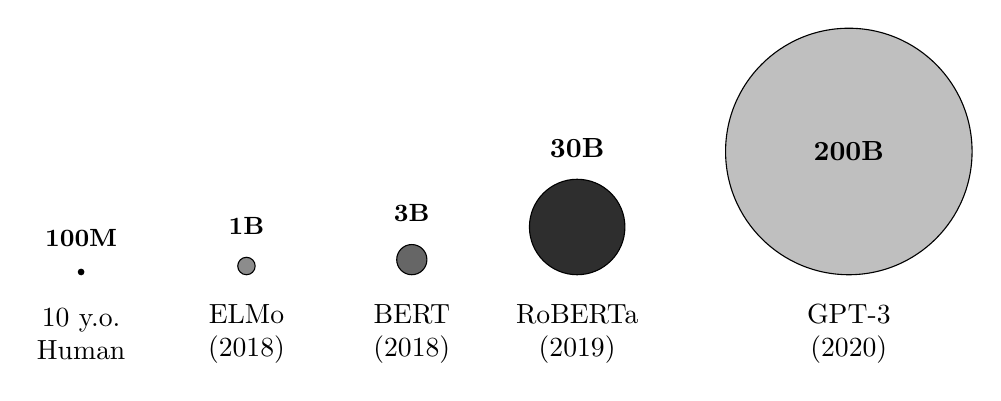
\begin{tikzpicture}[baseline]

% ---- Kreis 1: Human ----
%\def\rHuman{0.035} Fläche = 0.0038485
%\def\xHuman{1.0}
\def\rHuman{0.035}
\def\xHuman{1.0}
\draw[fill=black] (\xHuman,\rHuman) circle (\rHuman);
\node[align=center, font=\bfseries\small] at (\xHuman, 2*\rHuman+\valGap) {100M};
\node[align=center] at (\xHuman, -\capGap) {10 y.o.\\Human};

% ---- Kreis 2: ELMo ----
%\def\rElmo{0.053} This was wrong. Should be factor 10 of the Fläche 0.0038485 = 0.038485 -> r = 0.11068
%\def\xElmo{3.1}
\def\rElmo{0.11068}
\def\xElmo{3.1}
\draw[fill=black!45] (\xElmo,\rElmo) circle (\rElmo);
\node[align=center, font=\bfseries\small] at (\xElmo, 2*\rElmo+\valGap) {1B};
\node[align=center] at (\xElmo, -\capGap) {ELMo\\(2018)};

% ---- Kreis 3: BERT ----
%\def\rBert{0.092} % 3 Mal Fläche Elmo = 0,115455 -> r = 0.1917
%\def\xBert{5.2}
\def\rBert{0.1917}
\def\xBert{5.2}
\draw[fill=black!60] (\xBert,\rBert) circle (\rBert);
\node[align=center, font=\bfseries\small] at (\xBert, 2*\rBert+\valGap) {3B};
\node[align=center] at (\xBert, -\capGap) {BERT\\(2018)};

% ---- Kreis 4: RoBERTa ----
%\def\rRoberta{0.291} % 10 Mal Fläche Bert = 1,15455 -> r = 0.6062 
%\def\xRoberta{7.3}
\def\rRoberta{0.6062}
\def\xRoberta{7.3}
\draw[fill=black!82] (\xRoberta,\rRoberta) circle (\rRoberta);
\node[align=center, font=\bfseries] at (\xRoberta, 2*\rRoberta+\valGap) {30B};
\node[align=center] at (\xRoberta, -\capGap) {RoBERTa\\(2019)};

% ---- Kreis 5: GPT-3 ----
%\def\rGpt{0.751} % 6,66666 * Fläche Roberta = 7,697 r = 1.5653
%\def\xGpt{9.75}
\def\rGpt{1.5653}
\def\xGpt{10.75}
\draw[fill=black!25] (\xGpt,\rGpt) circle (\rGpt);
\node[align=center, font=\bfseries] at (\xGpt, \rGpt) {200B};
\node[align=center] at (\xGpt, -\capGap) {GPT-3\\(2020)};

\end{tikzpicture}}
\caption{Human input vs.\ size of training material for various LLMs.}\label{fig-training-data}
\end{figure}

\begin{figure}
% generated by Claude AI with figure in WB2022a as input and request to add Llama 3 data.
% Werte in Milliarden Tokens
% 10 y.o. Human : 0.1
% ELMo (2018)   : 1
% BERT (2018)   : 3
% RoBERTa (2019): 30
% GPT-3 (2020)  : 200
% Llama 3 (2024): 15000
% Radius proportional zu sqrt(Wert), Fläche also proportional zum Wert (Bubble-Chart-Konvention)
%
% Einheitlicher vertikaler Abstand zwischen Kreis und Bildunterschrift (unten)
% sowie zwischen Kreis-Oberkante und Wert-Label (oben, bei kleinen Kreisen)
\def\capGap{0.75}   % Abstand Baseline -> Bildunterschrift
\def\valGap{0.4}    % Abstand Kreis-Oberkante -> Wert-Label (kleine Kreise)
%
\oneline{%
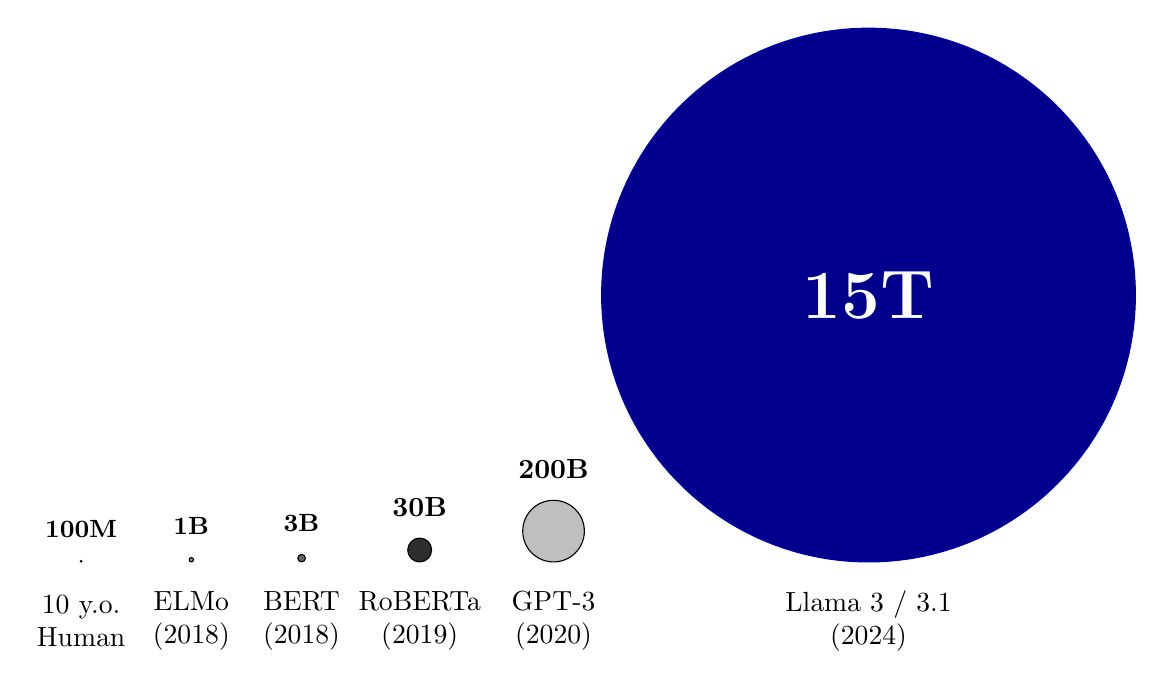
\begin{tikzpicture}[baseline]

% ---- Kreis 1: Human ----
%\def\rHuman{0.035} Fläche = 0.0038485
%\def\xHuman{1.0}
%\def\rHuman{0.035}
%\def\xHuman{1.0}
%\def\rHuman{0.0175}
\def\rHuman{0.00875}
\def\xHuman{1.0}
\draw[fill=black] (\xHuman,\rHuman) circle (\rHuman);
\node[align=center, font=\bfseries\small] at (\xHuman, 2*\rHuman+\valGap) {100M};
\node[align=center] at (\xHuman, -\capGap) {10 y.o.\\Human};

% ---- Kreis 2: ELMo ----
%\def\rElmo{0.053} This was wrong. Should be factor 10 of the Fläche 0.0038485 = 0.038485 -> r = 0.11068
%\def\xElmo{3.1}
%\def\rElmo{0.11068}
%\def\xElmo{3.1}
%\def\rElmo{0.05534}
\def\rElmo{0.02767}
\def\xElmo{2.4}
\draw[fill=black!45] (\xElmo,\rElmo) circle (\rElmo);
\node[align=center, font=\bfseries\small] at (\xElmo, 2*\rElmo+\valGap) {1B};
\node[align=center] at (\xElmo, -\capGap) {ELMo\\(2018)};

% ---- Kreis 3: BERT ----
%\def\rBert{0.092} % 3 Mal Fläche Elmo = 0,115455 -> r = 0.1917
%\def\xBert{5.2}
%\def\rBert{0.1917}
%\def\xBert{5.2}
\def\rBert{0.09585}
\def\rBert{0.047925}
\def\xBert{3.8}
\draw[fill=black!60] (\xBert,\rBert) circle (\rBert);
\node[align=center, font=\bfseries\small] at (\xBert, 2*\rBert+\valGap) {3B};
\node[align=center] at (\xBert, -\capGap) {BERT\\(2018)};

% ---- Kreis 4: RoBERTa ----
%\def\rRoberta{0.291} % 10 Mal Fläche Bert = 1,15455 -> r = 0.6062 
%\def\xRoberta{7.3}
%\def\rRoberta{0.6062}
%\def\xRoberta{7.3}
\def\rRoberta{0.3031}
\def\rRoberta{0.15155}
\def\xRoberta{5.3}
\draw[fill=black!82] (\xRoberta,\rRoberta) circle (\rRoberta);
\node[align=center, font=\bfseries] at (\xRoberta, 2*\rRoberta+\valGap) {30B};
\node[align=center] at (\xRoberta, -\capGap) {RoBERTa\\(2019)};

% ---- Kreis 5: GPT-3 ----
%\def\rGpt{0.751} % 6,66666 * Fläche Roberta = 7,697 r = 1.5653
%\def\xGpt{9.75}
%\def\rGpt{1.5653}
%\def\xGpt{10.75}
\def\rGpt{0.78265} % Fläche 1.9244
\def\rGpt{0.391325}
\def\xGpt{7}
\draw[fill=black!25] (\xGpt,\rGpt) circle (\rGpt);
\node[align=center, font=\bfseries] at (\xGpt, 2*\rGpt+\valGap) {200B};
\node[align=center] at (\xGpt, -\capGap) {GPT-3\\(2020)};


% ---- Kreis 6: Llama 3 (neu ergänzt) ----
%\def\rLlama{6.5}     % 75 * Fläche GPT = 577,275 r = 13.556
%\def\xLlama{16.0} % was 19.0
%\def\rLlama{13.556}
\def\rLlama{6.778}   % Fläche 144.33 = 75 * 1,9244 ok
\def\rLlama{3.389}   
\def\xLlama{11} % was 19.0
\draw[fill=blue!55!black, draw=blue!70!black] (\xLlama,\rLlama) circle (\rLlama);
\node[align=center, font=\bfseries\Huge, text=white] at (\xLlama, \rLlama) {15T};
\node[align=center] at (\xLlama, -\capGap) {Llama 3 / 3.1\\(2024)};
\end{tikzpicture}}
\caption{\citegen{WB2022a} figure of training data with addition of Llama 3}\label{fig-training-data-llama3}
\end{figure}
The figures display the training data of GPT-3. The size of the training data of more recent ChatGPT models is unknown but estimated to be much
bigger. \citet[6]{Lappin2024a} reports an estimation of a factor 6 for GPT-4. \citet{WB2022a} state that ChatGPT 3 had 20,000 years of human
input. For Llama 3 this would be 1,500,000 years. So, one can say that this differs quite dramatically from
human language acquisition.

\subsection{Grounding}

LLMs are trained on text. The words (or tokens for subparts of words) are not paired with semantic
knowledge. There is no relation to the ``real world''.
% \citep[11]{Lappin2024a} says that there is knowledge in them and that multi modal information can
% be provided. Yes, but this is what I argue as well. It has to be done.
\citet[358]{Piantadosi2024a} points out that semantic information is interwoven with syntactic
information. However,
the important point when it comes to human cognition is that the semantic knowledge in LLMs is not
grounded. \citet[1417]{JonesBergenTrott2024a} discuss sentence-picture verification tasks. For
example, hearers can infer from the sentences in (\mex{1}) that the nail is horizontal in the
situation described by the first sentence and vertical in the second. 
\eal
\ex He hammered the nail into the wall.
\ex He hammered the nail into the floor.
\zl
This information is not explicitly coded in the sentences, so LLMs, which are trained on language
  alone, cannot learn this, unless it is made explicit elsewhere in the training material.\footnote{%
See \citet{CM2001a} for computational experiments on language
  acquisition with grounding in the framework of Construction Grammar and \citet{Steels2003a} for
  experiments with grounded communication in robotics. \citet{BeulsVanEcke2024a} extensively
  discuss the shortcomings of LLMs that are due to their representations not being grounded and they
  suggest ways to model grounded language acquisition. \citet{JonesBergenTrott2024a} discuss first
  experiments with Multimodal LLMs and point out some shortcomings of current architectures.
\citet[11]{Lappin2024a} discusses Multimodal BERT and GPT-4, which was also trained on images during
a training phase called ``reinforcement learning based on the human feedback'' (RLHF).%
}
Therefore, it is really surprising to see Construction Grammarians
praising large language models as theories of human language. Construction Grammariens used to
emphasize the point that human cognition is grounded
\citep{Barsalou2008a} and that language is not just abstract
% Tomasello2003: Fillmore77, Fillmore77b, Langacker
syntax and hence, it cannot be learned as such without a connection to semantics and the real world
\parencites[44]{Klein86a-u}[113]{Tomasello2003a}[Section~4.2.3, 4.2.8]{AL2011a-u}{Clark2022a}. Grasping the communicative
intention and attention sharing\todostefan{\citet{Baldwin95a-u}} is considered
playing an important role in the acquisition process \parencites{Tomasello2003a}[134]{AL2011a-u,Clark2022a}[234]{Goldberg2024a}. Already in 1986, Klein pointed out that no human being could learn
Chinese by sitting in a room continually exposed to Chinese from loudspeakers.\footnote{%
This point is also acknowledged by \citet[234]{Goldberg2024a}.

Klein speculated that at most phonological regularities can be learned and \citet{NHSA2004a} showed
that humans can detect regularities by just being exposed to a continuous speech stream
of syllables of various forms. \citet[44]{Sogaard2023a} pointed out that two year old infants can learn
from TV, but TV involves another modality, the language is grounded \citep{Rice1983a}.
} This just would not work. But this is how LLMs learn: they just see masses and masses of
text. BERT was trained by guessing masked words in a sentence and by guessing the next
sentence. Children do not play such games. Instead, they have to solve a very hard puzzle on their own:
the segmentation of the speech signal. They have to find out what the units are in order to be able
to discover what they mean. 
% OK. This could be done in principle, the guessing game is more problematic, since it has nothing
% to do with human acquisition.
%
% Any theory of language acquisition has to take into account lifelong
% learning. Humans learn a language by using it. Since LLMs have clearly separated training and
% deployment phases they cannot be considered as ``the leading current theories of how speakers learn
% [\ldots] these restrictions'' \citet[\page 34]{AmbridgeBlything2024a}.\footnote{%
% I thank Remi van Trijp for pointing this out to me.} 
As \citet{BK2020a} pointed out: The early versions of BERT and ChatGPT and the like did not have a
clue about what they are ``saying'', since their linguistic information was not grounded
\citep{BeulsVanEcke2024a}. They often failed on very simple tasks like the \isi{Dumb Monty Hall
  Problem} \citep{Fraser2023a} and tasks for witch logical inferences are needed
\citep{CollinsThorneNewbury2026a}. % or tasks involving counting
Therefore pure text-based LLMs, the basic component of many AI systems, are often regarded as
bullshit machines \citep{HicksHumphriesSlater2024a}. The pure LLMs do not have a notion of truth and
no commitment to say true or false things. Their utterances are \emph{humbug} or
\emph{\isi{bullshit}} in the sense of \citet{Frankfurt1986a-u}. 



\subsection{Brain development}

As was pointed out in Section~\ref{sec-creols}, children regularize more than adults
\citep{HudsonN99a,HKN2005a}, a fact that can be traced back to their limited brain capacity (``less
is more''-hypothesis, \citealp{Newport90a,Elman93a}). Since large-scale commercial AI systems have other
purposes than modeling language acquisition, no such limitations are imposed in the training phase
of the involved LLMs.

\subsection{Interaction}

Language is acquired in interaction with shared attention
\parencites{Tomasello2003a}[134]{AL2011a-u,Clark2022a}[234]{Goldberg2024a}. \citet{CollinsThorneNewbury2026a} discuss
how values and group norms are formed. All this requires interaction and is fundamentally different
from reading the whole internet at once.

This means, if linguistics is dealing with human capabilities, we are not quite there yet. To
model language acquisition, we would need grounded input, we would need a realistic amount of
training data, we would have to simulate the development of brains and the growth of cognitive
capacities in early childhood. And we would need models involving interactions between speakers.



\subsection{But do we need LLMs for statements on Mainstream Generative Grammar?}

But what the success of LLMs suggests is that an elaborated component of Universal
Grammar is not needed, that the argument of the Poverty of the Stimulus was flawed and so on. Above
I wrote that ``we know no more about our cognitive abilities than we did before''. And this is
true. We knew in 1974 (50 years ago) that transformations are psycholinguistically
implausible \citep*[\page 320--328]{FBG74a-u}. Psycholinguists sympathetic with the Chomskyan paradigm suggested that we have our
linguistic knowledge represented as a Transformational Grammar, but that it then gets compiled out
into a set of templates that are equivalent ot the constructions of Construction Grammar \citep[\page 27]{FC96a-u}. But this
of course begs the question why one should not work in Construction Grammar or a related framework
like Constructional HPSG \citep{Sag97a,HPSGHandbook} from the beginning. What
is the evidence for some underlying transformation-based representation of linguistic knowledge? The
various architectures that were proposed over the years were psycholinguistically implausible
too. The T-Model \citep{Chomsky81a,Chomsky86b} was implausible (see Section~\ref{sec-incremental-processing}) and this got only worse with
Phase-based variants of Minimalism \parencites{Chomsky95a-u,Chomsky2008a}[\page 812,
830]{Richards2015a}[Section~5]{BM2021a}. But if the theories are incompatible with 
empirical facts like incremental processing, how can they tell us anything about human cognition and
inateness? 
% point later to DG article if it is published.
The Principle \& Parameter model of language acquisition \citep[\page 6]{Chomsky81a}
failed in various respects. It was assumed that one parameter was related to many properties of a
language and worked like a switch \parencites{Rizzi86a}[\page 8]{Chomsky2000a-u},
 but none of the suggested correlations held up (\cites{Haider94c-u}[Section~2.2]{Haider2001a}; see
 Section~\ref{section-PP} of this book for an overview).
The way
parameterization was conceptualized was biologically implausible. For example, it was assumed that
Subjacency was a universal principle and the parameterization concerned the part of speech of
certain bounding nodes within nonlocal dependencies \parencites[\page 271]{Chomsky73a}[\page 40]{Chomsky86b}{Baltin81a,Baltin2006a}.
First, it could be shown that Subjacency does not hold in
Dutch, German and English \parencites[\page 52]{Koster78b-u}[\page
211]{Mueller99a}{Mueller2004d}[Section~3]{Mueller2007c}{SS2013b-u} and second, it is biologically
absolutely implausible that part of speech information is encoded in our genes \parencites{Bishop2002a}[Section~6.4.2.2]{Dabrowska2004a}{FM2005a}.
This was realized by
\citet*{HCF2002a}. What remained as property that was assumed to be part of Universal Grammar was
Merge, an operation for combining linguistic material. Somehow a triviality (see
p.\,\pageref{ex-n-ary-merge}). A triviality that caused another linguistic war \citep{Pullum2024a}.\nocite{Harris93a}
 
There is one important aspect of research in the Principles \& Parameters era: The systematic search for
universals, for commonalities and differences lead to a much improved knowledge about variation. We
know much more about language as such, that is, about structures that are similar in principle.
For example, the German sentence in (\ref{ex-quietschen}) is parallel to the English translation. 
\ea
\label{ex-quietschen} 
\gll dass die Straßenbahnen um die Ecke quietschen\\
     that the trams         around the corner squeak\\
\glt `that the trams squeak around the corner'
\z
As \citet{MuellerUnifying} pointed out, it is possible to develop analyses that capture the
commonalities although the linearization of the constituents differs in German and English (English
is an SVO language and German is SOV). \citet{MuellerLFGphrasal} developed accounts of the
benefactive construction and the resultative construction that work for English and German, although
these languages differ in various ways also affecting these constructions.
Typological research is fascinating and requires the comparison of many very different languages on a
theoretical level. I doubt that the results of cross-linguistic research can be derived from LLMs,
without any interaction with theoretical linguistics. Training LLMs on multilingual material will be
non-trivial\footnote{
  See \citet{ChangArnettTu2024a} for comments on the low quality of multilingual language
  models. Note also that a lot of typologically interesting languages are low-resource languages, so
  a massive training like with current commercial LLMs is not possible because of the lack of data. See
  \citet{ChangArnettTu2024a} on monolingual models for 350 languages.
} and discovering cross-linguistic generalizations in network representations is probably
impossible without a theoretically informed clue on what to look for (see also
footnote~\ref{fn-dependencies} on p.\,\pageref{fn-dependencies}). A suggestion for a
methodological clean way of deriving cross-linguistic generalizations that differs from the MGG
approach is assumed in the CoreGram project \citep{MuellerCoreGram}.

Chomsky claimed that there would be language universals but there are no plausible candidates for
syntactic universals left (\citealt{EL2009a}; see Section~\ref{sec-syntactic-universals} for an overview). There are tendencies, for sure, but this is not sufficient for positing
innate knowledge of language. 
%Recently, I discovered a universal, but it is not syntactic but rather
%on the text level: the Festschrift Universal. The reader is referred to \citew{MuellerFestschrift}
%for details.


The strongest argument for innate linguistic knowledge seemed to be the Argument from the Poverty of the Stimulus, but
it was never actually correctly carried out \citep{PS2002a,SP2002b}. Chomsky repeated his favourite argument
with question formation as auxiliary inversion throughout several decades \parencites[\page 29--33]{Chomsky71a-u}[\page 39]{Chomsky2013a}. \citet{Bod2009a} showed
how frequencies of subtrees can be used to learn structures of auxiliary inversion even though the
examples that Chomsky (wrongly\footnote{%
See \citet[\page 41--45]{PS2002a}.
}) claimed to be non-existent in the input to children were not used in the training data. Chomsky
ignored these insights (\citealt*{BPYC2011a}, \citealt[\page 39]{Chomsky2013a}) and so we 
find the auxiliary inversion claim again two years later in the same journal that also published Bod's paper.
Similarly pattern-based modeling language acquisition research was much more successful in explaining
cross-linguistic differences in acquisition than alternative accounts couched in Chomskyan
frameworks \citep{FPG2006a,FPAG2007a,FPG2009a}.
%\citeauthor{Bod2009a} and \citeauthor{FPG2006a} assume that there is structure, though. 


Connected to the assumption of Universal Grammar is the assumption of a core/""periphery
distinction \parencites[\page 7--8]{Chomsky81a}[\page 150--151]{Chomsky86a}[\page 343]{Fodor98a}. The idea is that there is a core of linguistic knowledge that is determined by our
genetic endowment and there is a periphery (e.\,g. idioms) that is learned in another way. There is an interesting and very
simple argument against this stance and it goes like this: If we can learn the idiosyncratic parts of a language that is
assigned to the periphery, we should be able to learn the more regular parts of the assumed core
\parencites[\page 20]{Abney96a}[\page 222]{Goldberg2003b}[\page 14]{Goldberg2006a}[\page 100]{Newmeyer2005a}[\page 36]{Tomasello2006a}[\page
20]{Tomasello2006c}{MuellerKernigkeit}. 
See \citew{MuellerKernigkeit} and the CoreGram project \citep{MuellerCoreGram}
for a method for deriving language-internal and also cross-linguistic generalizations and the notion
of \emph{Kernigkeit} (coriness) that does not refer to Chomsky's core/periphery distinction. 

So, we knew that Chomskyan approaches to language and language acquisition failed in terms of their
basic assumptions (transformations), they failed in terms of their architecture with respect to
psycholinguistic evidence (separation of syntax and phonology and semantics in various forms) and
they failed in respect to assumptions about genetics. Everybody working in non-Chomskyan paradigms
has been aware of this for more than a decade (see the first editions of my \emph{Grammatical
  theory} textbook from 2010 and 2014 for a summary of the respective discussions in German and
English, respectively). We did not need LLMs for this, but maybe the actual usefulness of these
networks is that they make it plausible to linguists and laymen that we do not need any innate
domain-specific knowledge. However, to show that LLMs can acquire languages like humans do, they
have to be more human-like. To reach this goal, we probably need more knowledge about brains. As I
pointed out above, if we manage to reach the goal of creating more human-like models, we know how
brains work, but we do not necessarily know how languages work.

I mentioned many of the failures of Chomskyan theories above, but note that they were very
successful. They contributed to our understanding of language. The reason is that they were
theories. They made predictions and contained claims about languages. We knew how to falsify them
and we did. The era of research on Principles \& Parameters was fruitful in that it caused a
enormous amount of typological research. LLMs on the other hand are black boxes. They make
predictions, some right, some wrong, but this is all we have. There is no explicit law that is falsified.

A further note is necessary here: Piantadosi claimed that the existence of LLMs shows that there is
no Poverty of the Stimulus, but as \citet[6]{Baroni2023a} argued, current LLMs are not blank
slates. Their architectures make very specific assumptions and hence have certain biases. The fact
that LLMs with different architectures learn different things is evidence of this. So it is
possible in principle that they have some bias towards hierarchical structure and without such bias
language would not be learnable. So the way forward seems to be to experiment with different
architectures, to experiment with different datasets and sizes of datasets to find out what is
needed. \citet{WB2022a} describe this in more detail. Pointing at large scale commercial LLMs for
proof of concept is not legitimate, since too many of their properties are unrealistic for human
language acquisition or unknown and not modifiable.

\section{Linguistic theories}
\label{sec-linguistic-theories}

I believe that linguistic theories should contain rules and symbols. A linguistic theory can to some
extent be derived from large corpora using automatic methods. Both the categories can be obtained
via class formation and rules or valence patterns and the corresponding lexical entries can be
derived automatically. The parts of speech and features like case, gender and
number that are currently used in linguistic theories are basically the outcome of a distributional
analysis that was done ``by hand'' during the last centuries. Grammar rules and also feature-value
pairs may be assigned probabilities \citep{Jurafsky96a}. These can also be derived from corpora. This is complicated and
the mathematics is not fully understood yet. But one can train the system on large amounts of
data. The training procedure contains assumptions about language: there are categories, there are
constituents. There will be a residuum of infrequent phenomena that will not be captured
this way (for example apparent multiple frontings, see \citealt{Mueller2003b}). Some fine-tuning will be
required and this is where the linguist comes in: rare data and complicated interacting phenomena may decide between various alternative
theories of a language \citep[Chapter~6]{MuellerGS}. 
%
% Chinesisch https://www.youtube.com/watch?v=xLg9M_mKrxU

\if0
\section{LLMs and linguistic experiments}
\label{sec-LLMs-experiments}

I perceive the current situation in theoretical linguistics this way: there are basically two
camps. One is basically Mainstream Generative Grammar. Proponents follow a certain school of
thinking and style of grammar writing. Some assume Universal Grammar, some do not and some are
agnostic. On the other side we have Construction Grammar or usage-based grammar. Many formal
frameworks team up with Construction Grammar. Now, many researchers from the Construction Grammar
camp embrace LLMs and think that they basically are what they always thought grammatical theories
should be, while many MMG linguists utterly reject LLMs.

The question is: how can LLMs be useful for linguists? What do they show? Some linguists use LLMs
for experiments rather than doing experiments with humans. The advantage of LLMs is that they can be
asked anytime, they do not cost as much as people. Whether LLM experiments are useful strongly
depends on how the experiments are done (which is also true for experiments with humans
\ldots). Some linguists ask LLMs to judge sentences on a Likert skale. This is strange since it
means that the LLM gets a task that it tries to solve based on probabilities assigned to this
question. We as users do not know whether the AI systems that are questioned this way have ways to
react to our requests that involve additional steps, but if we just rely on pure LLMs, asking for
ratings would be strange indeed. What can be done though is measuring surprisal via a special
interface to LLMs.

\citet{Catasso2026a-u} run experiments with humans and with LLMs (direct question, not via an
interface) and compared the results. In most cases the LLM behaved like the human subjects. This is
a good result, but Catasso also found cases in which the LLMs differed from
humans. 
% \citet{Webelhuth2026a} showed that the information encoded in LLMs differs from what we know
% about humans, since LLMs cannot do embeddings under control verbs. This means that there may be
% situations in which LLMs differ from humans and hence, all experiments based on LLMs have to be
% verified with human subjects. The question is whether it is useful at all to do LLM-based
% experiments.

The other extreme is MGG linguists who want to show that LLMs do not contain their
theories (\eg \citealt{MurphyLeivadaDentella2025a-u}). \citet{MurphyLeivadaDentella2025a-u} write:\footnote{
  Note that the bracketing [a [stubbornly [resilient wall]]] is in the abstract of the paper. I
  think it should have been [a [[stubbornly resilient] wall]], since \emph{stubornly} modifies
  \emph{resilient} since it is an adverb rather than an adjective. Claude AI, ChatGPT and Google AI
  got the bracketing right on 05.09.2026.
}
\begin{quote}
In stark contrast to many recent claims that artificial language models are on the verge of
replacing the field of linguistics, our results suggest not only that deep learning is hitting a
wall with respect to compositionality (Marcus, 2022), but that it is hitting [a [stubbornly
[resilient wall]]] that cannot readily be surmounted to reach human-like compositional reasoning
simply through more compute. \citep[1--2]{MurphyLeivadaDentella2025a-u}
\end{quote}
In order to do so, they ask LLMs or rather AI systems containing LLMs for theoretical analyses and
celebrate if they cannot provide one. For example, \citet[11]{MurphyLeivadaDentella2025a-u} use the following prompt:
\ea
Draw me a syntactic tree structure, in line with Minimalist syntax,
for the sentence `The doctor the nurse the hospital had hired met John'.
\z
% Create for me a semantic or philosophical paradox that is more
% complex and sophisticated than all existing paradoxes or puzzles.
% Task is inconsistent: If sentences are ungrammatical and theory is correct, there should not be trees.
%
% Generate two sentences. The first sentence must contain one type
% of syntactic violation. The second sentence must continue the discourse
% content from the first, but must contain a different type of
% syntactic violation that explicitly is caused by some type of relation
% or connection with the first sentence. Draw a Minimalist tree structure
% to map the explicit coordination of these multiple error types.
The authors go on and ask for complex example sentences involving ungrammaticality. What is asked
for is some meta level reflection. But this is quite a specialized task and most humans would not be
able to draw a syntactic tree in any version of a Chomskyan theory. I am teaching students who try
very hard and fail. Yet, they master the German language. So, the claim that LLMs correspond to some
theory of language (Usage-based Construction Grammar, Dependency Grammar) is quite different from
the claim that LLMs can do the same as linguists. The experiments of
\citet{MurphyLeivadaDentella2025a-u} are as if one would ask a young adult to explain the grammar
they are using. Most will not be able to do this. LLMs may have learned something about MMG by reading papers
about Generative Grammar, but since there are so many different approaches and some are mutually
inconsistent and some others are even internally inconsistent, the likelyhood of an LLM producing a
coherent MGG story is probably not that high. In any case, this is not what usage-based linguist
meant when they were saying LLMs are a theory of language.
\fi



\section{Conclusion}
\label{sec-LLMs-conclusion}

Large Language Models are not theories of language. To build LLMs, one needs a theory and depending
on the goal to be reached, the theory may be a theory of the human brain. Knowing how a brain works does not entail knowledge about language. To do typological research means to compare
thousands of languages. This is done by theoretical linguists on a meta level and not within
neuronal nets trained with input of thousands of languages. Of course, one can imagine typological
research supported by computers, but it would require trained linguists who know what to look for.
The existence and success of LLMs does not entail
that the problem of human language acquisition is solved, since the architecture and the training
process of LLMs is quite different from how human brains develop and how humans acquire
language. However, LLMs show that the data is rich and make it even more plausible that humans are
not born with innate domain specific knowledge about language.

%\itdopt{\citet{RooijGuestAdolfi2024a-u}}

\furtherreading{
This chapter is based on \citew{MuellerLLMs}.
}


%      <!-- Local IspellDict: en_US -->

% Goldberg2024
% Finally, there is evidence that humans spontaneously predict the next word
% that will be uttered while comprehending language (e.g., Kutas & Federmeier
% 2011). For instance, the N400 ERP component, detectable from EEG recordings
% on the scalp while people listen to text, correlates quite well with how predictable
% each word is in context